\documentclass[12pt, a4paper]{report}


\usepackage{anyfontsize}
\usepackage{titlesec}
\usepackage{graphicx}
\usepackage{refstyle}
\usepackage{amsfonts}
\usepackage{amsmath}
\usepackage{placeins}
\usepackage{flafter}




% Title Page
\title{FRA501 Class Project: 1-Dimension Jumping Robot}
\author{Chawakorn Chaichanawirote, Kanut Thummaraksa, 
	\\and Noppasorn Larpkiattaworn}


\begin{document}
\maketitle
We model and simulate the dynamics and control of a 1-dimension Jumping robot with a linear actuator.\par
\section*{Robot Model}
\subsection*{Continuous Dynamics}
The robot consists of two links; a linear actuator with mass $m_a$ and a moving thrust rod $m_r$. The bottom of the rod is connected to a massless spring, with a stiffness of $k$ and a drag coefficient $b$. Figure \ref{fig:system} shows the system diagram.

%% System Fig
\begin{figure}[h]
	\vspace{1pt}
	\centering
	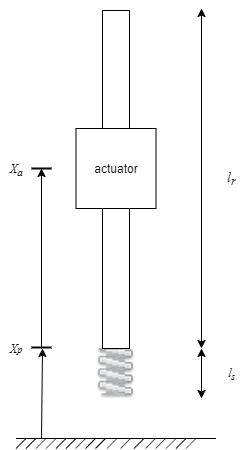
\includegraphics[scale=0.6]{images/JumpingRobot.png} 
	\caption{The jumping robot.}
	\label{fig:system}
\end{figure}\par

The joint space of the robot is defined by

\begin{equation}
	\vec{q} = \begin{bmatrix}
	x_{p}\\
	x_{a}
	\end{bmatrix}
\end{equation}
We use Lagrangian dynamics to model the system's behaviour. Note that for convenience's sake, we will consider the spring force as an external force, as the links in motion must be rigid bodies\par
The Lagrangian $\mathcal{L}$ of a mechanical system is defined by a the difference between its kinetic and potential energy
\begin{equation}
\mathcal{L} = K - P
\end{equation}
\begin{equation}
	\mathcal{L} = \frac{1}{2}m_{a}(\dot{x_{a}} + \dot{x_{p}})^{2}+\frac{1}{2}m_{r}\dot{x_{p}}^{2}-m_{a}g(x_{a}+x_{p})-m_{r}g(x_{p}+\frac{l_{r}}{2})
\end{equation}

The Euler-Lagrange equations are then

\begin{equation}
	\frac{d}{dt}\frac{\partial L}{\partial \dot{\vec{q}}} - \frac{\partial L}{\partial \vec{q}} = Su
	\label{eq:euler-lagrange}
\end{equation}
where,
$S$ is the selection matrix of the input $u$. For this robot, $S = \begin{bmatrix}
0&1
\end{bmatrix}$\par 
The input force given by the actuator is $u = F_{a}$. From (\ref{eq:euler-lagrange}) and the Lagrangian, we have

\begin{equation}
\begin{bmatrix}
m_{a} + m_{r}&0\\
0 & m_{a}
\end{bmatrix}
\begin{bmatrix}
\ddot{x_{p}}\\
\ddot{x_{a}}
\end{bmatrix}
+\begin{bmatrix}
m_{a}+m_{r}\\m_{a}
\end{bmatrix}g =
\begin{bmatrix}
0\\1
\end{bmatrix}
F_{a}
\label{eq:ballistic}
\end{equation}

With no external force acting on the system, (\ref{eq:ballistic}) represents the dynamics of the robot in mid-air. Once the spring touches the ground($x_{p}<l_{s}$)and starts to compress, we can add its external force $f_{s} = -(k(l_{s}-x_{p})+b\dot{x_{p}})$ to the system via its transposed Jacobian $J_{s}^{T} = \begin{bmatrix}
1\\0
\end{bmatrix}$ to get

\begin{equation}
\begin{bmatrix}
m_{a} + m_{r}&0\\
0 & m_{a}
\end{bmatrix}
\begin{bmatrix}
\ddot{x_{p}}\\
\ddot{x_{a}}
\end{bmatrix}
+\begin{bmatrix}
m_{a}+m_{r}\\m_{a}
\end{bmatrix}g =
\begin{bmatrix}
0\\1
\end{bmatrix}
F_{a} - 
\begin{bmatrix}
1\\0
\end{bmatrix}
(k(l_{s}-x_{p})-b\dot{x_{p}})
\label{eq:ground}
\end{equation}

(\ref{eq:ground}) represents the dynamics of the system when the robot is on the ground. This can be generalized into the robot equation
\begin{equation}
	M\vec{a} + G = S\vec{u} + J_{s}^{T}f_{s}
\end{equation}

\subsection*{Discrete States}

 The robot's actuation of $x_{a}$ has a limit of $[0, l_{r}]$, at the limits, we can classify the sytem's behaviour into four constrained states. At this point, we introduce a discrete valued state variable $x_{d} \in \{0, 1, 3, 4, 5\} \subset \mathbb{Z}$ that encodes the contact situations as assigned in Figure \ref{fig:contactdiagram}.\par

%% Contact Diagram Fig
\begin{figure}[h]
	\vspace{1pt}
	\centering
	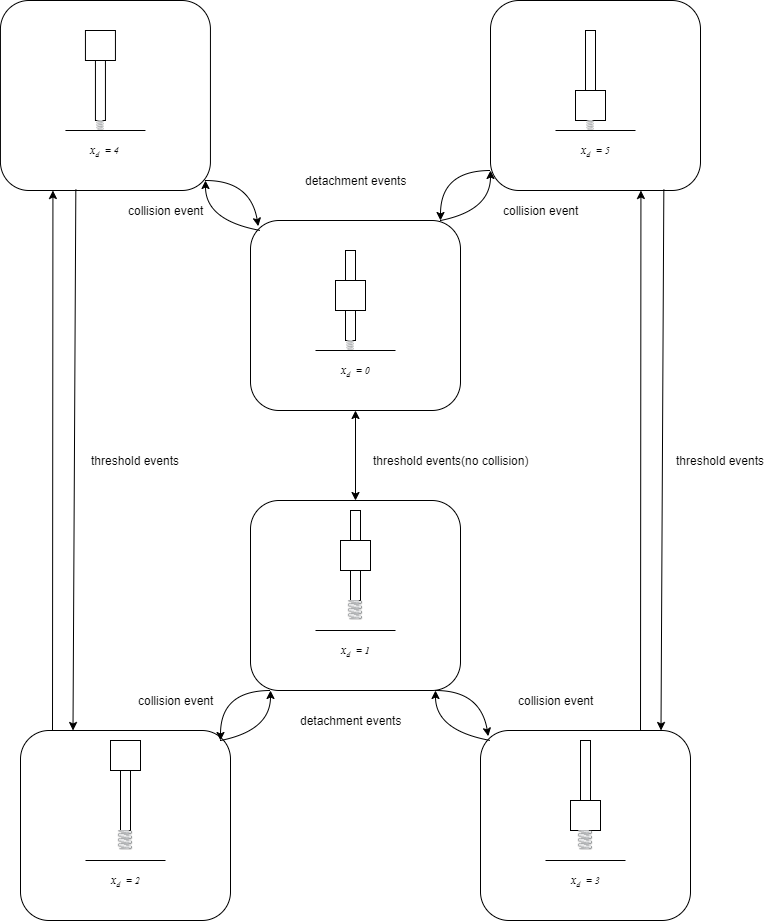
\includegraphics[scale=0.6]{images/transitiongraph.png} 
	\caption{Transition graph of the robot.}
	\label{fig:contactdiagram}
\end{figure}
\FloatBarrier

The contact force for each contact situation is 

\begin{equation}
	F_{c} = (J_{c}M^{-1}J_{c}^{T})^{-1}(J_{c}M^{-1}G - J_{c}M^{-1}S\vec{u} - J_{c}M^{-1}J_{s}^{T}f_{s})
\end{equation}

Which allows us to find the acceleration

\begin{equation}
	\vec{a} = M^{-1}(-G+S\vec{u} + J_{s}^{T}f_{s} + J_{c}F_{c})
\end{equation}

The Jacobian for all contacts are $J_{c} = \begin{bmatrix}
0 & 1
\end{bmatrix}$. Note that $f_{s}$ is only present for states with $x_{p}<l_{s}$.\par 
Next, we find the the collision force of each collision, $F_{i}$, as well as the velocity after impact of the actuator $v^{+}$

\begin{equation}
F_{i} = -(J_{c}M^{-1}J_{c}^{T})^{-1}J_{c}v^{-}
\end{equation}

\begin{equation}
	v^{+} = v^{-} + M^{-1}(J_{c}^{T}F_{i})
\end{equation}

With these equations, we can simulate the dynamics of the robot.


\section*{Simulation}
We implement the simulation and control in MATLAB, using according to the following control diagram.

%% Control Diagram Fig
\begin{figure}[h]
	\vspace{1pt}
	\centering
	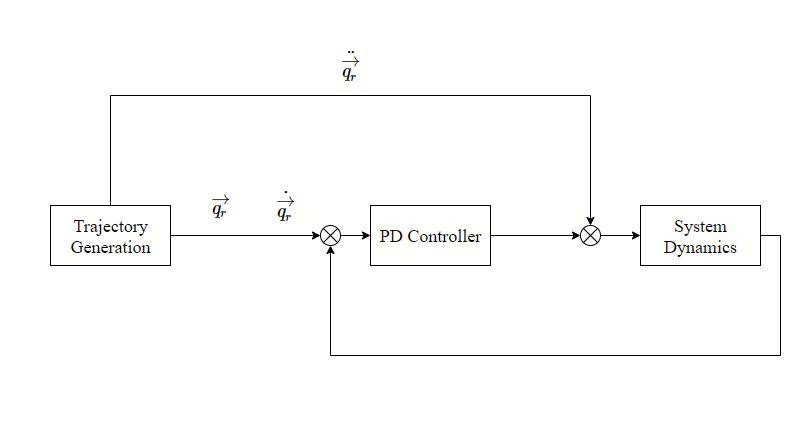
\includegraphics[scale=0.7]{images/system.jpg} 
	\caption{Control of the robot.}
	\label{fig:blockdiagram}
\end{figure}\par
We run the simulation using the following input trajectory.
$$\vec{q} = \frac{l_{r}}{2}(2\pi t)+\frac{l_{r}}{2}$$
$$\dot{\vec{q}} = 2\pi\cos(2\pi t)$$
$$\ddot{\vec{q}} = -4\pi^{2}(\frac{l_{r}}{2})\sin(2\pi t)$$
The PD constants are $K_{p} = 1000, K_{d} = 10$\par
The system is simulated for total time $T = 30 $ seconds. The initial values and constants are as follows(all units are SI):\par 
$$x_{a} = 0.25$$
$$x_{p} = 10.2$$
$$x_{d} = 1$$

$$g = 9.80665$$
$$m_{r} = 0.2$$
$$m_{a} = 1$$
$$l_{s} = 0.2$$
$$l_{r} = 0.5$$

The results of the simulation are shown in Figure \ref{fig:result}.

%% Result Fig
\begin{figure}[h]
	\vspace{1pt}
	\centering
	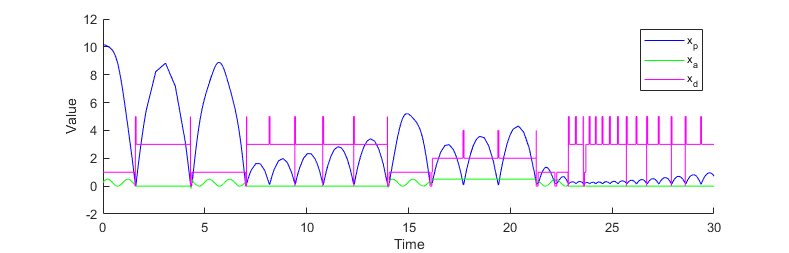
\includegraphics[scale=0.8]{images/simulation.png} 
	\caption{The result of the simulation.}
	\label{fig:result}
\end{figure}\par

Notice that the robot achieves a jumping motion, while the values for $x_{a}$ are still within its bounds.

\end{document}          
